% ***************************************************
% Example of Figures
% ***************************************************
%This example is provided for your reference only. DO NOT INCLUDE IN YOUR FINAL THESIS. 

%\begin{figure} : If you put no command after \begin{table} then this figure will be printed anywhere in your pdf where LaTex finds the free space to put it. If you wish to specify where the figure goes you have to give a command in LaTex after  \begin{figure}. 
%
%There are different commands to put the figure in different positions e.g. \begin{table}[h] LaTex will print the figure in the same position that you put it in your source file, if there is enough space to print it
%N.B. it is important to note that commanding LaTeX to add a figure in a specific place may result in formatting issues.

\chapter{Example of Figures}

\begin{figure}[h]
\begin{center}
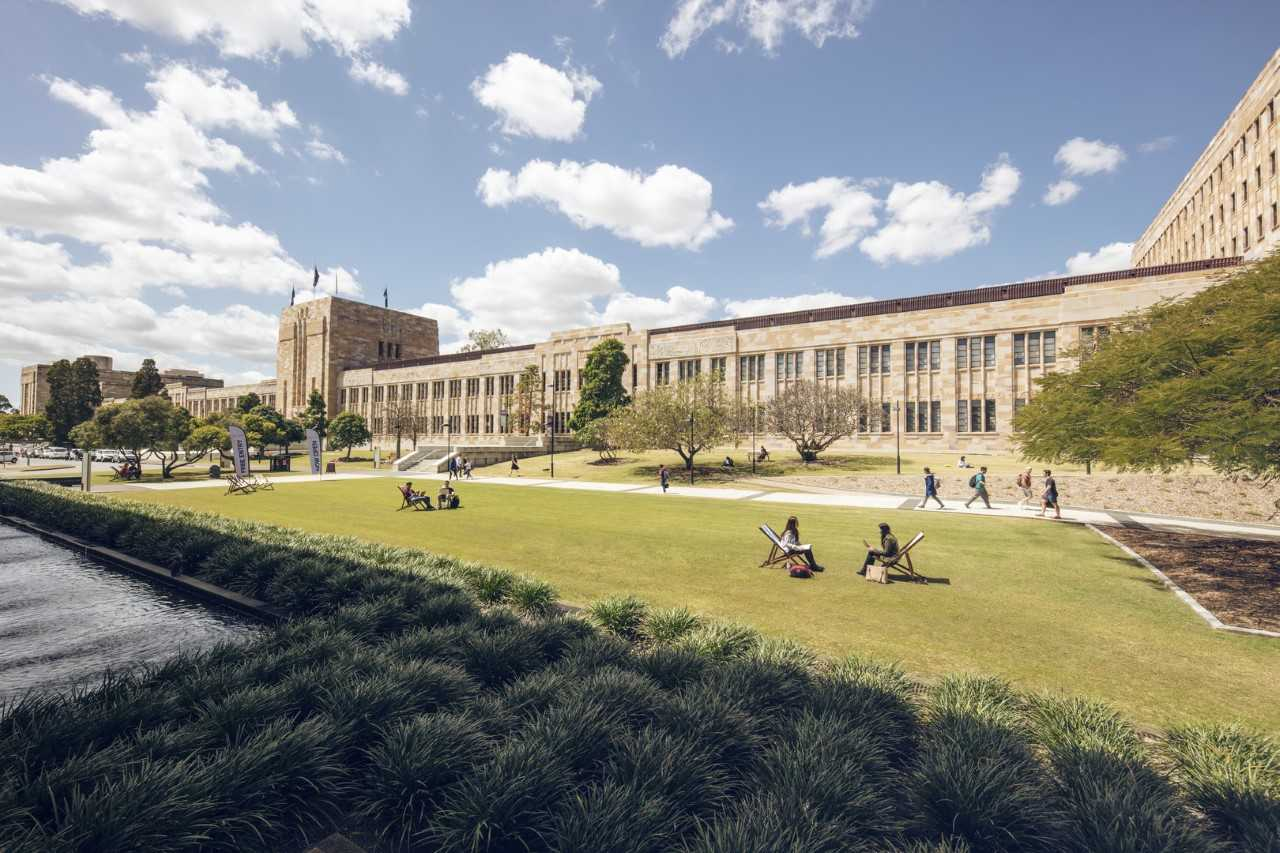
\includegraphics[width=1.0\textwidth]{Examples/FigureUQ}
\caption{The University Of Queensland}
\label{Fig:1}
\end{center}
\end{figure}

The Figure~\ref{Fig:1} represents beauty of the UQ campus.